\documentclass{article}
\usepackage[utf8]{inputenc}
\usepackage{subfiles}
\usepackage{lscape}
\usepackage[a4paper, total={6in, 8in}]{geometry}
\usepackage{hyperref}
\usepackage{natbib}
\usepackage{graphicx}

\graphicspath{{images/}{../images/}}


\title{Dokumentation Abschlussprojekt WEBLAB \\
        \textbf{Travelblog}}
\author{Patrick Marty (tamarty)}
\date{HS19, 02.03.2020}

\begin{document}
\maketitle


\vspace{2cm}
\begin{figure}[h]
        \centering
        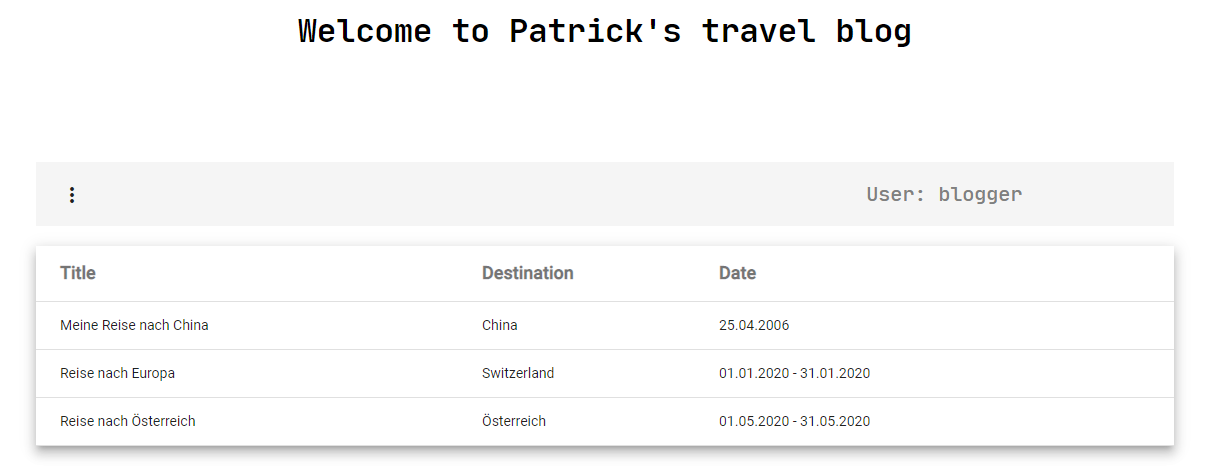
\includegraphics[width=1\textwidth]{blogDashboard.png}
\end{figure}

\vspace{1cm}

\section{Einführung}\label{einfuhrung}
\subfile{Einfuhrung/einfuhrung}
\footnote{Frontend Applikation: \url{https://github.com/martypa/weblab-travelblog.git}}
\footnote{Backend Applikation:  \url{https://github.com/martypa/travelblog-backend.git}}
\footnote{Dokumentation:        \url{https://github.com/martypa/weblab-dokumentation.git}}
\newpage

\section{Architektur}\label{architektur}
\subfile{Architektur/architektur}

\vspace{2cm}
\section{Backend}\label{backend}
\subfile{Backend/backend}

\section{Frontend}\label{frontend}
\subfile{Frontend/frontend}

\section{Fazit \& Reflexion}\label{fazit}
\subfile{Fazit/fazit}
\newpage

\begin{landscape}
\section{Arbeitsjournal}\label{arbeitsjournal}
\subfile{arbeitsjournal}
\end{landscape}

\end{document}
